\documentclass[11pt,a4paper]{article}

% =========================================================================
%   TRANSIT ACCESSIBILITY CONCEPT PAPER & RESEARCH COMPENDIUM
%   Sudirman Corridor, South Jakarta & Jabodetabek Urban Transit Scope
%   Prepared for Overleaf Collaborative Sharing & Research Distribution
%   Tim Riset Pijak & Apple Developer Academy Team
% =========================================================================

% ------------------------- Core Encodings & Fonts ------------------------
\usepackage[utf8]{inputenc}
\usepackage[T1]{fontenc}
\usepackage{lmodern}

% ------------------------- Page Geometry & Layout ------------------------
\usepackage[a4paper,top=1in,bottom=1in,left=1in,right=1in]{geometry}
\usepackage{setspace}
\onehalfspacing

% ------------------------- Mathematics & Symbols -------------------------
\usepackage{amsmath,amssymb,amsfonts}

% ------------------------- Tables & Figures ------------------------------
\usepackage{booktabs}
\usepackage{tabularx}
\usepackage{longtable}
\usepackage{array}
\usepackage{multirow}
\usepackage{caption}
\usepackage{float}

% ------------------------- Visual & Colors -------------------------------
\usepackage{xcolor}
\usepackage{graphicx}
\usepackage{tcolorbox}
\tcbuselibrary{skins,breakable}

% ------------------------- TikZ Diagrams ---------------------------------
\usepackage{tikz}
\usetikzlibrary{shapes.geometric,arrows.meta,positioning,calc,fit,backgrounds,decorations.pathreplacing}

% ------------------------- Lists & Typography ----------------------------
\usepackage{enumitem}
\usepackage{microtype}
\usepackage{titlesec}
\usepackage{fancyhdr}

% ------------------------- Hyperlinks ------------------------------------
\usepackage[hidelinks,colorlinks=true,linkcolor=pijakblue,citecolor=pijakblue,urlcolor=pijakteal]{hyperref}

% ------------------------- Color Definitions -----------------------------
\definecolor{pijakblue}{HTML}{1A365D}      % Deep Navy
\definecolor{pijakteal}{HTML}{0D9488}      % Teal Accent
\definecolor{pijakamber}{HTML}{D97706}     % Warm Warning/Hazard
\definecolor{pijakred}{HTML}{DC2626}       % Critical Failure / Barrier
\definecolor{pijakgray}{HTML}{4B5563}      % Muted Gray
\definecolor{pijaklight}{HTML}{F3F4F6}     % Card Background
\definecolor{pijakborder}{HTML}{E5E7EB}    % Subtle Border
\definecolor{pijakgreen}{HTML}{16A34A}     % High Accessibility / Shade

% ------------------------- Section Formatting ----------------------------
\titleformat{\section}
  {\Large\bfseries\color{pijakblue}}
  {\thesection}{0.8em}{}
\titleformat{\subsection}
  {\large\bfseries\color{pijakblue}}
  {\thesubsection}{0.6em}{}
\titleformat{\subsubsection}
  {\normalsize\bfseries\color{pijakteal}}
  {\thesubsubsection}{0.5em}{}

\titlespacing*{\section}{0pt}{1.5em}{0.6em}
\titlespacing*{\subsection}{0pt}{1.2em}{0.4em}
\titlespacing*{\subsubsection}{0pt}{0.9em}{0.3em}

% ------------------------- Header & Footer -------------------------------
\pagestyle{fancy}
\fancyhf{}
\renewcommand{\headrulewidth}{0.4pt}
\renewcommand{\footrulewidth}{0.4pt}
\fancyhead[L]{\small\textcolor{pijakgray}{\textbf{Transit Accessibility Concept Paper} $\vert$ Research Banks \& Routing}}
\fancyhead[R]{\small\textcolor{pijakgray}{Tim Riset Pijak -- Sept 2026}}
\fancyfoot[L]{\small\textcolor{pijakgray}{Overleaf Concept Edition -- Jabodetabek Scale}}
\fancyfoot[R]{\small\thepage}

% ------------------------- Callout Box Styles ----------------------------
\newtcolorbox{conceptbox}[2][]{
  enhanced,
  colback=pijaklight,
  colframe=pijakblue,
  fonttitle=\bfseries\color{white},
  coltitle=white,
  colbacktitle=pijakblue,
  title=#2,
  arc=3mm,
  boxrule=0.8pt,
  left=8pt,right=8pt,top=8pt,bottom=8pt,
  #1
}

\newtcolorbox{hazardbox}[2][]{
  enhanced,
  colback=white,
  colframe=pijakamber,
  fonttitle=\bfseries\color{white},
  coltitle=white,
  colbacktitle=pijakamber,
  title=#2,
  arc=2mm,
  boxrule=1pt,
  left=8pt,right=8pt,top=8pt,bottom=8pt,
  #1
}

\newtcolorbox{databankbox}[2][]{
  enhanced,
  colback=pijaklight,
  colframe=pijakteal,
  fonttitle=\bfseries\color{white},
  coltitle=white,
  colbacktitle=pijakteal,
  title=#2,
  arc=2mm,
  boxrule=0.8pt,
  left=8pt,right=8pt,top=8pt,bottom=8pt,
  #1
}

% =========================================================================
%   DOCUMENT METADATA
% =========================================================================
\title{%
  \vspace{-1.5cm}
  {\Huge\bfseries\color{pijakblue} Beyond the Pavement Edge:}\\[0.3em]
  {\Large\bfseries\color{pijakteal} A 4-Pillar Multimodal Routing Engine, Computational Spatial Pipeline, and Targeted Field Research Architecture for Inclusive Transit in Greater Jakarta}\\[0.6em]
  {\normalsize\color{pijakgray} Comprehensive Research Bank, Empirical Field Data Synthesis, and Product Strategy}
}

\author{%
  \textbf{Gading Aditya Perdana}$^{1}$, \textbf{Kenrich Heavenly Sandria}$^{1}$, \textbf{Naufal Ammar Rauf}$^{1}$,\\
  \textbf{Jatayu Muhammad Wicaksono}$^{1}$, \textbf{Sintani Gina Lestari}$^{1}$\\[0.5em]
  \small $^{1}$Tim Riset Pijak / Apple Developer Academy @ BINUS Cohort 8--9\\
  \small In Collaboration with Urban Community Partners: Wisma Cheshire Indonesia \& Jakarta Barrier Free Tourism\\
  \small \texttt{\{gading.perdana, team\}@pijak-research.org}
}

\date{\textbf{September 2026} $\vert$ Version 2.4 (Overleaf Ready)}

% =========================================================================
\begin{document}
% =========================================================================

\maketitle
\thispagestyle{fancy}

\begin{abstract}
\noindent
Urban mass rapid transit systems in developing megacities frequently succeed at moving millions along high-capacity trunks, yet fail catastrophically at the pedestrian last-mile. In Greater Jakarta (Jabodetabek), despite massive capital investments in MRT, LRT, and BRT networks, pedestrian mode share remains below two percent. This concept paper synthesizes four months of empirical investigation across the Sudirman transit corridor and broader South Jakarta, documenting the systemic failure modes of commercial routing systems (Google Maps, Apple Maps) for pedestrians, women at night, and citizens with permanent physical disabilities. We present a three-stage methodological evolution: from early manual corridor audits (June 2026), to the native baseline accessibility prototype (\emph{Pijak}, July 2026), to a scalable automated spatial computing framework (September 2026) combining aerial semantic segmentation (\texttt{Tile2Net}), street-level computer vision (\texttt{Mapillary/SegFormer}), and solar microclimate shadow modeling (\texttt{CoolWalks}). 

\noindent
To resolve the fundamental failure of distance-minimizing navigation, we formally introduce the \textbf{4-Pillar Routing Model}: (1) \textbf{Fastest} (multimodal chaining across ojol, feeder, and rail), (2) \textbf{Comfort} (dynamic thermal shade routing, passive nocturnal surveillance, and physiological walk caps), (3) \textbf{Cheapest} (a Rupiah tariff engine exploiting Rp~0 JakLingko, Rp~3,000 KRL, and Rp~3,500 Transjakarta fare integration), and (4) \textbf{Wheelchair Accessible} (strict step-free topological graph certainty). Crucially, to prevent wasteful over-auditing, we establish a rigorous \textbf{Field Research Decision Framework} that defines exactly what can and must be automated via remote sensing versus where in-situ field research is strictly mandatory: micro-validation of multi-level vertical transit choke points, user co-testing with permanent wheelchair residents from Wisma Cheshire, and active-learning ground-truthing of high-disagreement model predictions. This document serves as the canonical research bank, technical specification, and collaborative baseline for academic and municipal stakeholders.
\end{abstract}

\vspace{0.5em}
\noindent\textbf{Keywords:} Urban Accessibility, Pedestrian Network Modeling, Multimodal Chaining, Thermal Comfort, Wheelchair Navigation, Computer Vision, Tile2Net, CoolWalks, Wisma Cheshire, Jakarta Transit.

\vspace{0.8em}
\hrule
\vspace{1em}

% =========================================================================
\section{Executive Summary \& Research Trajectory}
% =========================================================================

Jakarta presents one of the most stark pedestrian paradoxes in Southeast Asia. While the Jalan Jenderal Sudirman corridor was extensively re-engineered between 2017 and 2022 into a showcase boulevard with sidewalks up to 12 meters wide, complete with landscaped buffers and multi-transit interchanges, pedestrian commute mode share city-wide remains stalled at under 2\% \cite{itdp2019, goodstats2024}. Prior corridor studies documented acceptable perception scores on revitalized segments \cite{dwisadana2024, apritasari2020satisfaction} alongside pedestrian volume gains following road-diet initiatives \cite{mulyadi2022, ridhani2015}. Yet at major transit hubs such as Dukuh Atas, last-mile friction and access barriers persist \cite{rakhmatulloh2020, napitupulu2025tod}. The city operates roughly 540~km of engineered sidewalk against more than 6,956~km of roadway---a pedestrian network coverage of less than 8\%.

\begin{figure}[H]
\centering
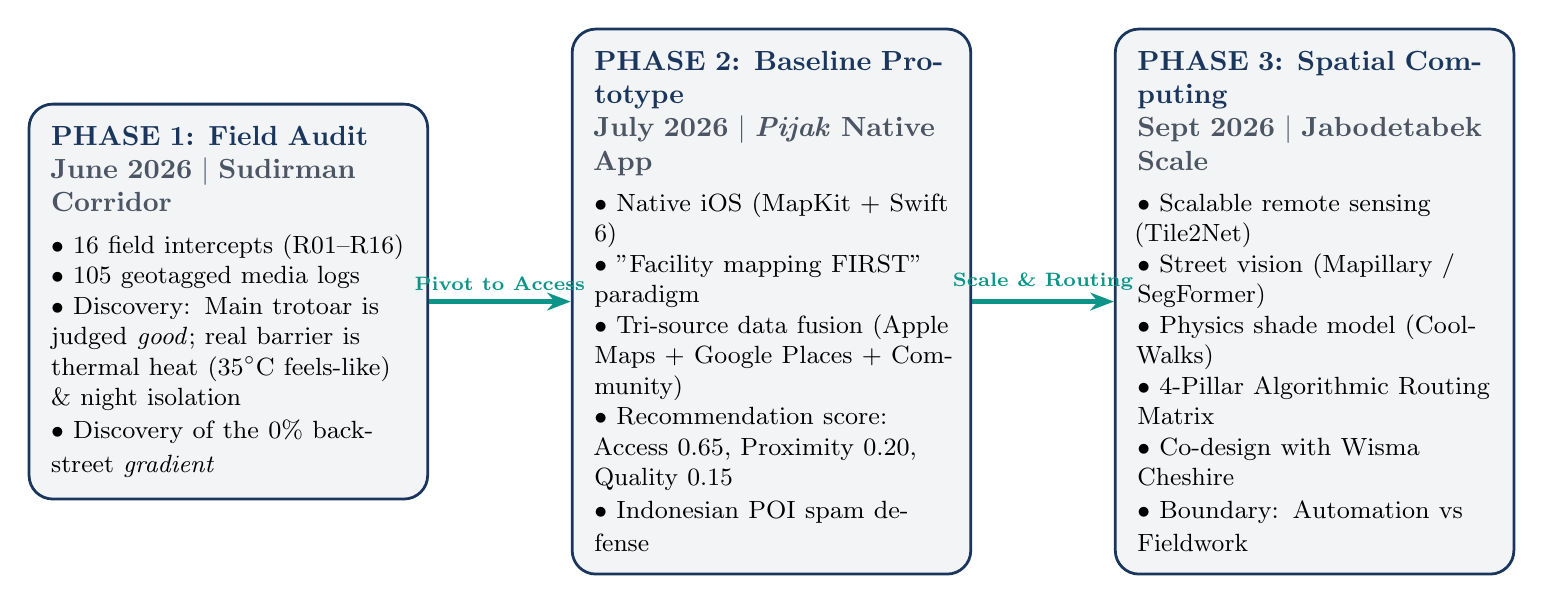
\begin{tikzpicture}[
    node distance=1.2cm and 1.8cm,
    phase/.style={rectangle, rounded corners=3mm, draw=pijakblue, fill=pijaklight, line width=1pt, text width=4.5cm, minimum height=3.8cm, align=left, inner sep=8pt},
    header/.style={font=\bfseries\color{pijakblue}, align=center},
    arrow/.style={-{Stealth[length=3mm]}, line width=1.5pt, draw=pijakteal}
]
    % Node Phase 1
    \node (p1) [phase] {
        \textbf{\color{pijakblue}PHASE 1: Field Audit}\\
        \textbf{\color{pijakgray}June 2026 $\vert$ Sudirman Corridor}\\[0.4em]
        \small $\bullet$ 16 field intercepts (R01--R16)\\
        $\bullet$ 105 geotagged media logs\\
        $\bullet$ Discovery: Main trotoar is judged \emph{good}; real barrier is thermal heat (35$^\circ$C feels-like) \& night isolation\\
        $\bullet$ Discovery of the 0\% back-street \emph{gradient}
    };
    
    % Node Phase 2
    \node (p2) [phase, right=of p1] {
        \textbf{\color{pijakblue}PHASE 2: Baseline Prototype}\\
        \textbf{\color{pijakgray}July 2026 $\vert$ \emph{Pijak} Native App}\\[0.4em]
        \small $\bullet$ Native iOS (MapKit + Swift 6)\\
        $\bullet$ "Facility mapping FIRST" paradigm\\
        $\bullet$ Tri-source data fusion (Apple Maps + Google Places + Community)\\
        $\bullet$ Recommendation score: Access 0.65, Proximity 0.20, Quality 0.15\\
        $\bullet$ Indonesian POI spam defense
    };
    
    % Node Phase 3
    \node (p3) [phase, right=of p2] {
        \textbf{\color{pijakblue}PHASE 3: Spatial Computing}\\
        \textbf{\color{pijakgray}Sept 2026 $\vert$ Jabodetabek Scale}\\[0.4em]
        \small $\bullet$ Scalable remote sensing (Tile2Net)\\
        $\bullet$ Street vision (Mapillary / SegFormer)\\
        $\bullet$ Physics shade model (CoolWalks)\\
        $\bullet$ 4-Pillar Algorithmic Routing Matrix\\
        $\bullet$ Co-design with Wisma Cheshire\\
        $\bullet$ Boundary: Automation vs Fieldwork
    };

    % Arrows
    \draw [arrow] (p1) -- (p2) node [midway, above, font=\scriptsize\bfseries\color{pijakteal}] {Pivot to Access};
    \draw [arrow] (p2) -- (p3) node [midway, above, font=\scriptsize\bfseries\color{pijakteal}] {Scale \& Routing};
\end{tikzpicture}
\caption{The three-stage research and engineering evolution of Tim Riset Pijak (June--September 2026).}
\label{fig:evolution_timeline}
\end{figure}

The transition across these three phases revealed crucial structural lessons:
\begin{enumerate}[leftmargin=1.5em]
    \item \textbf{Debiasing the Urban Narrative (Phase 1):} Our initial hypothesis assumed pedestrians walk in the street because sidewalks are physically broken. Fieldwork completely dismantled this: pedestrians rated the main Sudirman sidewalk as \emph{"enak, lega, manusiawi"} (pleasant, spacious, humane). The true operational barriers were \emph{environmental heat} (ambient 33$^\circ$C, feels-like 35$^\circ$C, UV index 8), \emph{micro-hazard drop-offs} at zebra crossings, and nocturnal \emph{spatial isolation} ("terang tapi sepi").
    \item \textbf{The Facility-First Architecture (Phase 2):} In developing the native iOS prototype \emph{Pijak}, caregiver interviews and accessibility experts established that turn-by-turn routing is secondary to \textbf{threshold certainty}. For a wheelchair user or elderly citizen, arriving at a destination that lacks a ramp, elevator, or accessible restroom results in complete mission failure. We codified an accessibility score weighting facility completeness at 0.65 over proximity at 0.20.
    \item \textbf{The Scale Impasse and Algorithmic Generalization (Phase 3):} A team of five field researchers required three weeks to audit a single 3.5~km stretch of Sudirman. Manual auditing cannot scale across Greater Jakarta's 6,956~km road network. In Phase 3, we architected an automated remote sensing and computer vision pipeline, paired with a 4-pillar multiobjective routing engine and a formal decision matrix governing in-situ human validation.
\end{enumerate}

% =========================================================================
\section{The Empirical Research Data Banks}
% =========================================================================

The findings and algorithmic parameters implemented in our architecture rest upon five primary data banks collected, ingested, and maintained within our research workspace.

\subsection{Data Bank 1: Ground-Truth Field Intercepts (R01--R16 \& Notulen)}
On 18 June 2026, two coordinated field teams conducted structured, neutral intercepts along the Sudirman spine (Dukuh Atas to Semanggi), capturing 12 complete audio interviews, 12 observational notulen entries, 105 geotagged multimedia records, and concurrent microclimate readings (Apple WeatherKit).

\begin{table}[H]
\centering
\small
\caption{Selected Field Intercepts and Ground-Truth Insights (Sudirman Corridor Audit).}
\label{tab:field_intercepts}
\renewcommand{\arraystretch}{1.2}
\begin{tabularx}{\textwidth}{l p{3.2cm} p{2.2cm} c c p{4.2cm}}
\toprule
\textbf{ID} & \textbf{Role / Persona} & \textbf{Location} & \textbf{Sec.$^a$} & \textbf{Comf.$^a$} & \textbf{Ground-Truth Signal \& Key Pain Point} \\
\midrule
R01 & Area Security Guard & MRT/KAI Dukuh Atas & 6 & 7 & Jurisdictional gap between KAI, MRT, and National Police; public zone outside gates is unpoliced. \\
R02 & Daily Commuter & Jl. Raya Sudirman & 9 & 8 & Extreme midday sun exposure; mature tree buffer compensates; trotoar judged spacious. \\
R03 & Counter-Commuter & Halte Dukuh Atas & 8 & 6 & Demands continuous physical canopy; feels safer when pedestrian flow is quiet. \\
R04 & Elderly Daily Walker & Sarinah--Semanggi & 9 & 9 & Walks 1.5h daily for health; reassured by police posts; heat acute near Sarinah/Embassy. \\
R05 & Transjakarta Commuter & CSW--Setiabudi & 7 & 6 & Kerb-to-zebra cross ramp drop-off is excessively steep/slippery; friend fell twice; carries umbrella. \\
R06 & High School Students (2) & Palmerah--SMAN 3 & 9 & 9 & High safety perceived in groups; no catcalling experienced on broad arterial footways. \\
R07 & Motorcyclist & Sudirman Parking & 8 & 7 & Avoids midday walking entirely due to heat; enjoys walking only after dark. \\
R08 & MITJ Transit Worker & Stasiun Sudirman & 8 & 8 & TOD construction creates temporary bottlenecks; former begal/crime hotspot neutralized. \\
R09 & JPO Night Security & JPO Upper Deck & 5 & 7 & Upper bridge deck deserted after 22:00; "Terang tapi sepi" (lit but empty = high fear). \\
R10 & Father with Child & Sudirman Spine & 8 & 7 & Kerb ramp drop-off too abrupt for strollers; fast vehicles turning into side streets. \\
R11 & Urban Planning Critic & Sudirman Walkway & 7 & 4 & \textbf{Design critique:} Copied 4-season European templates; no sun canopy; foliage blocks lamps at night. \\
R12 & Mobile Satpol PP & Polda--Summitmas & 6 & 8 & Ojol riding onto sidewalk; jurisdictional deadlock (motorcycles = Dishub remit; Satpol PP = PKL). \\
N11 & Kendal Tunnel Guard & Terowongan Kendal & -- & -- & Tripping on uneven pavement joints; complaints submitted to provincial CRM ignored. \\
N12 & Local Resident (Ibu Lis) & Kendal Area & -- & -- & Chronic broken tactile paving; reports to JAKI ignored; feels municipal apathy. \\
\bottomrule
\multicolumn{6}{l}{\footnotesize $^a$ Security and Comfort scores are analyst-interpreted scales (1--10) from grounded qualitative transcripts.}
\end{tabularx}
\end{table}

\subsection{Data Bank 2: Spatial Facility Layer (\texttt{dukuh\_atas\_facilities.geojson})}
Targeting the multimodal Dukuh Atas Transit Interchange bbox ($106.817^\circ\text{E}$ to $106.828^\circ\text{E}$, $-6.208^\circ\text{S}$ to $-6.197^\circ\text{S}$), we extracted and mapped 235 distinct physical infrastructure features.

\begin{conceptbox}{The OpenStreetMap Accessibility Void}
Our programmatic audit of the OpenStreetMap (OSM) dataset covering the Dukuh Atas TOD hub revealed a catastrophic blind spot in global collaborative GIS:
\begin{itemize}[leftmargin=1.5em]
    \item \textbf{Mapped Features (235 Total):} Pedestrian Paths: 114 $\vert$ Zebra/Signal Crossings: 58 $\vert$ Engineered Sidewalks: 56 $\vert$ Vertical Elevators: 4 $\vert$ Drinking Water Fountains: 2 $\vert$ Public Toilets: 1.
    \item \textbf{Unmapped / Completely Missing in OSM:} \textbf{0 Public Benches} $\vert$ \textbf{0 Wheelchair-Accessible Toilets} (\texttt{toilets:wheelchair=yes}) $\vert$ \textbf{0 Tactile Paving Ways} (\texttt{tactile\_paving=yes}).
\end{itemize}
\emph{Conclusion:} Commercial and open-source mapping engines assume that if a transit station exists, it is accessible. In reality, essential accessibility features are invisible in primary spatial databases.
\end{conceptbox}

\subsection{Data Bank 3: Routable Pedestrian Network (\texttt{pedestrian\_network.geojson})}
Spanning the arterial spine between Bundaran HI and Semanggi, this OpenSidewalks-aligned spatial database contains \textbf{680 topologically connected features}:
\begin{itemize}[leftmargin=1.5em]
    \item \textbf{Traversable Edges:} 317 dedicated footways, 143 street-adjacent sidewalks, 88 road crossings, and 20 pedestrian overpasses (JPO) and multi-level skybridges.
    \item \textbf{Point Barriers \& Amenities:} 105 physical barriers (bollards spaced $<0.80\text{ m}$, unauthorized vendor lockouts, steep kerbs), 4 public toilets, 2 transit shelters, and 1 mapped resting bench.
\end{itemize}

\subsection{Data Bank 4: POI Directory (\texttt{dukuh\_atas\_places.csv})}
A curated directory of \textbf{111 high-traffic Points of Interest (POIs)} located within an 800-meter walk shed of the Dukuh Atas nexus. Categorized into:
\begin{itemize}[leftmargin=1.5em]
    \item \textbf{Financial \& Banking (14 POIs):} Bank Mandiri, BCA, BNI, BRI, Permata, HSBC, ICBC.
    \item \textbf{Essential Convenience (7 POIs):} 24-hour convenience stores (Alfamart, Indomaret, FamilyMart, Lawson) serving as lighting anchors and informal emergency shelters.
    \item \textbf{Food, Beverage \& Community (90 POIs):} Ranging from Difabis Coffee and Tea (operated by baristas with hearing and physical disabilities) to multi-tenant commercial centers.
\end{itemize}

\subsection{Data Bank 5: The Walkability Gradient Index (\texttt{gradient.csv})}
The most profound empirical contribution of our spatial analysis is the quantification of the \textbf{Walkability Gradient}---the extreme spatial disparity between the revitalized arterial avenue and the unmanaged urban kampungs immediately behind it.

\begin{table}[H]
\centering
\small
\caption{The Walkability Gradient: Arterial Showcase vs. Back-Street Realities (69 Streets Audited).}
\label{tab:gradient_comparison}
\renewcommand{\arraystretch}{1.2}
\begin{tabularx}{\textwidth}{l r r c p{4.5cm}}
\toprule
\textbf{Street Name} & \textbf{Total Len. (m)} & \textbf{Sidewalk Len. (m)} & \textbf{Coverage (\%)} & \textbf{Pedestrian Reality \& Infrastructure} \\
\midrule
\multicolumn{5}{l}{\textbf{\color{pijakteal}Arterial Showcase \& Primary Connectors (100\% Sidewalk Coverage -- 21 Streets Total)}} \\
Jl. Martapura & 196.5 & 196.5 & \textbf{100.0\%} & Broad paved walkway, tactile guides, tree canopy. \\
Jl. Talang Betutu & 290.5 & 290.5 & \textbf{100.0\%} & Paved sidewalk, protected bollards, residential buffer. \\
Jl. Bendungan Hilir & 1,444.7 & 1,444.7 & \textbf{100.0\%} & Commercial spine sidewalk, moderate vendor activity. \\
Jl. K.H. Mas Mansyur & 1,199.1 & 1,199.1 & \textbf{100.0\%} & Major flyover underpass sidewalk, heavy traffic buffer. \\
Jl. Setiabudi Raya & 305.4 & 305.4 & \textbf{100.0\%} & Standard sidewalk, commercial frontage. \\
\midrule
\multicolumn{5}{l}{\textbf{\color{pijakamber}Transition Corridors (60\% -- 75\% Sidewalk Coverage -- 3 Streets Total)}} \\
Jl. Kendal & 583.9 & 424.3 & \textbf{72.7\%} & Pedestrianized tunnel zone; broken joints at fringes. \\
Jl. Teluk Betung & 168.8 & 120.8 & \textbf{71.6\%} & Sidewalk discontinues near commercial access gates. \\
Jl. Blora & 259.3 & 160.3 & \textbf{61.8\%} & High culinary pedestrian density; kerbs blocked by ojol. \\
\midrule
\multicolumn{5}{l}{\textbf{\color{pijakred}The Forgotten Urban Fabric (0.0\% Sidewalk Coverage -- 45 Streets Total)}} \\
Jl. Karet Pedurenan Raya & 676.5 & 0.0 & \textbf{0.0\%} & Pedestrians forced into dense mixed traffic. \\
Jl. Kebon Sayur & 311.5 & 0.0 & \textbf{0.0\%} & Narrow residential lane; open roadside gutters (\emph{got}). \\
Gang Kebon Kacang XLIV & 165.7 & 0.0 & \textbf{0.0\%} & Dense kampung alley; motorcycles parked on edges. \\
Jl. Dukuh Pinggir V & 279.2 & 0.0 & \textbf{0.0\%} & Primary shortcut from KRL station; 0 sidewalk. \\
Jl. Perintis & 335.5 & 0.0 & \textbf{0.0\%} & High wall perimeter; unlit ditch; extreme night hazard. \\
Jl. Administrasi & 398.9 & 0.0 & \textbf{0.0\%} & Direct hospital feeder road; zero pedestrian walkway. \\
\bottomrule
\end{tabularx}
\end{table}

\noindent
\textbf{Quantitative Gradient Finding:} Out of 69 named streets audited within the Sudirman core buffer, \textbf{65.2\% (45 streets) have exactly 0.0\% sidewalk coverage}. This creates an insurmountable barrier for active mobility: the moment a commuter steps 50 meters off the main avenue, the pedestrian environment collapses into vehicular conflict.

% =========================================================================
\section{Google Maps Teardown: Failure Modes in Developing Cities}
% =========================================================================

Mainstream navigation engines (Google Maps, Apple Maps) were engineered primarily for vehicular optimization and later adapted for pedestrians using planar distance minimization. In dense Southeast Asian transit ecosystems, this architecture produces systemic failures.

\begin{figure}[H]
\centering
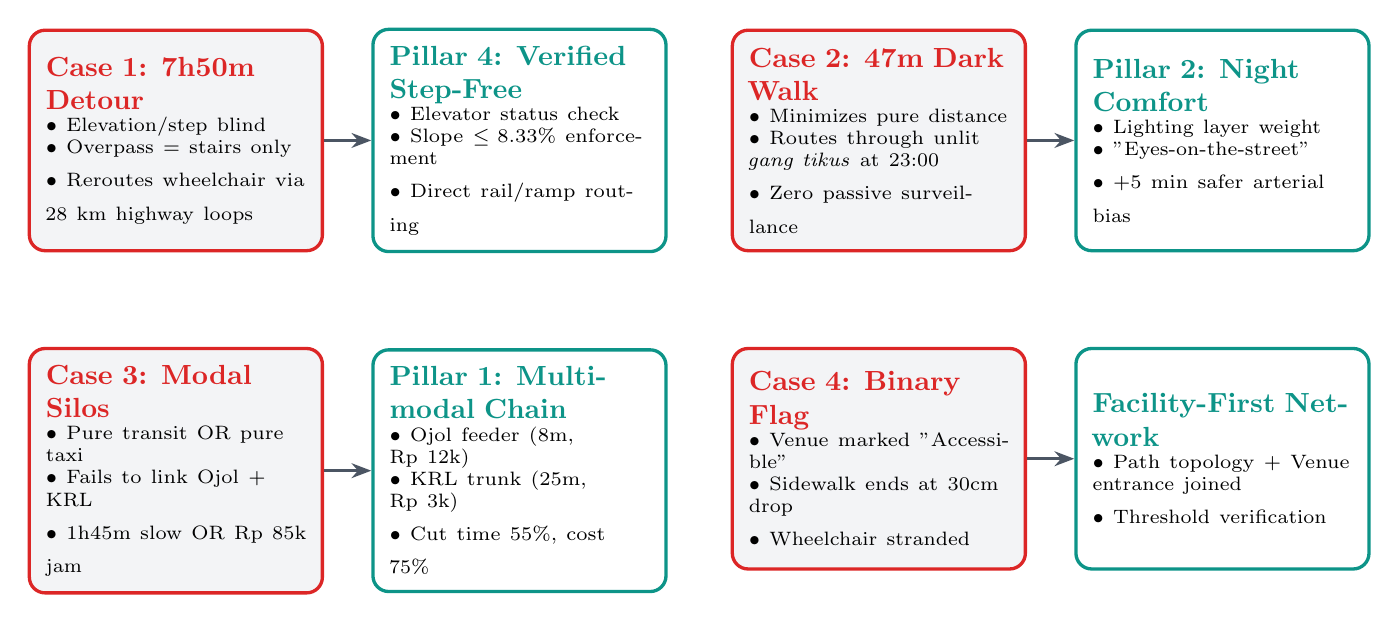
\begin{tikzpicture}[
    box/.style={rectangle, rounded corners=2mm, draw=pijakblue, fill=white, line width=1pt, text width=3.3cm, minimum height=2.8cm, align=left, inner sep=6pt},
    badbox/.style={rectangle, rounded corners=2mm, draw=pijakred, fill=pijaklight, line width=1.2pt, text width=3.3cm, minimum height=2.8cm, align=left, inner sep=6pt},
    solbox/.style={rectangle, rounded corners=2mm, draw=pijakteal, fill=white, line width=1.2pt, text width=3.3cm, minimum height=2.8cm, align=left, inner sep=6pt},
    lbl/.style={font=\bfseries\small\color{pijakblue}, align=center},
    arr/.style={-{Stealth[length=2.5mm]}, line width=1.2pt, draw=pijakgray}
]
    % Rows
    \node (c1) [badbox] {
        \textbf{\color{pijakred}Case 1: 7h50m Detour}\\
        \scriptsize $\bullet$ Elevation/step blind\\
        $\bullet$ Overpass = stairs only\\
        $\bullet$ Reroutes wheelchair via 28~km highway loops
    };
    \node (s1) [solbox, right=0.6cm of c1] {
        \textbf{\color{pijakteal}Pillar 4: Verified Step-Free}\\
        \scriptsize $\bullet$ Elevator status check\\
        $\bullet$ Slope $\le 8.33\%$ enforcement\\
        $\bullet$ Direct rail/ramp routing
    };

    \node (c2) [badbox, right=0.8cm of s1] {
        \textbf{\color{pijakred}Case 2: 47m Dark Walk}\\
        \scriptsize $\bullet$ Minimizes pure distance\\
        $\bullet$ Routes through unlit \emph{gang tikus} at 23:00\\
        $\bullet$ Zero passive surveillance
    };
    \node (s2) [solbox, right=0.6cm of c2] {
        \textbf{\color{pijakteal}Pillar 2: Night Comfort}\\
        \scriptsize $\bullet$ Lighting layer weight\\
        $\bullet$ "Eyes-on-the-street"\\
        $\bullet$ +5 min safer arterial bias
    };

    \node (c3) [badbox, below=1.2cm of c1] {
        \textbf{\color{pijakred}Case 3: Modal Silos}\\
        \scriptsize $\bullet$ Pure transit OR pure taxi\\
        $\bullet$ Fails to link Ojol + KRL\\
        $\bullet$ 1h45m slow OR Rp~85k jam
    };
    \node (s3) [solbox, right=0.6cm of c3] {
        \textbf{\color{pijakteal}Pillar 1: Multimodal Chain}\\
        \scriptsize $\bullet$ Ojol feeder (8m, Rp~12k)\\
        $\bullet$ KRL trunk (25m, Rp~3k)\\
        $\bullet$ Cut time 55\%, cost 75\%
    };

    \node (c4) [badbox, below=1.2cm of c2] {
        \textbf{\color{pijakred}Case 4: Binary Flag}\\
        \scriptsize $\bullet$ Venue marked "Accessible"\\
        $\bullet$ Sidewalk ends at 30cm drop\\
        $\bullet$ Wheelchair stranded
    };
    \node (s4) [solbox, right=0.6cm of c4] {
        \textbf{\color{pijakteal}Facility-First Network}\\
        \scriptsize $\bullet$ Path topology + Venue entrance joined\\
        $\bullet$ Threshold verification
    };

    \draw [arr] (c1) -- (s1);
    \draw [arr] (c2) -- (s2);
    \draw [arr] (c3) -- (s3);
    \draw [arr] (c4) -- (s4);
\end{tikzpicture}
\caption{Deconstruction of Google Maps commercial navigation failures and our architectural remedies.}
\label{fig:gmaps_teardown}
\end{figure}

\subsubsection{Case Study 1: The 7-Hour-50-Minute Airport Wheelchair Detour}
When a mobility-impaired user requests wheelchair-accessible transit directions from Sudirman to Soekarno-Hatta Airport or across the railway corridor at Karet, Google Maps exhibits severe topological failure. Because its planar street graph lacks step-vs-ramp vertical tagging on footbridges (JPOs), it flags pedestrian crossings as physically impassable. However, instead of identifying a nearby station elevator or low-floor feeder, the routing algorithm calculates a circuitous \textbf{7-hour-50-minute (34 km) walking detour} along arterial shoulders, or fails completely.

\subsubsection{Case Study 2: The 47-Minute Unlit Suburban Night Walk}
Standard pedestrian navigation operates on a static cost objective:
\begin{equation}
    \min \sum_{e \in \text{Path}} \frac{\text{length}(e)}{v_{\text{walk}}}
\end{equation}
At 23:00 WIB, a commuter arriving at an outer suburban rail terminal (e.g., Rawa Buntu, Jurang Mangu, or Manggarai fringe) is routinely directed into a \textbf{47-minute walk through completely unlit back-alleys (\emph{gang tikus})}, deserted canal banks, and blind corners with zero commercial activity. Google Maps saves 4 minutes of walking time at the expense of severe vulnerability to mugging (\emph{begal}) and physical injury from open drainage pits.

\subsubsection{Case Study 3: The Multimodal Chaining Breakdown (Ojol + Rail Disconnect)}
In Greater Jakarta, over 70\% of daily commuters live in suburban residential clusters located 3 to 10~km from the nearest KRL Commuter Line station. Google Maps forces a binary choice:
\begin{itemize}[leftmargin=1.5em]
    \item \textbf{Option A (Pure Transit):} Walk 45 mins to an infrequent local bus $\rightarrow$ transfer twice $\rightarrow$ KRL. Total travel time: \textbf{1 hour 50 minutes}.
    \item \textbf{Option B (Pure Rideshare):} Point-to-point Gojek/GrabCar directly to central Jakarta. Fare: \textbf{Rp~75,000--95,000}; caught in 45-minute congestion chokepoints along Tol Jagorawi or Rasuna Said.
\end{itemize}
Google Maps completely fails to compute the optimal multi-modal chain: \textbf{8-minute Ojol to station drop-off (Rp~12,000) + 28-minute KRL Express (Rp~3,000) + 5-minute walk}. This hybrid route costs only Rp~15,000 and slashes commute time to 41 minutes.

% =========================================================================
\section{The 4-Pillar Algorithmic Routing Model}
% =========================================================================

To resolve the systemic failures of commercial engines, we formulate a generalized multiobjective routing model operating on a directed spatial graph $G = (V, E)$. The edge set $E$ is partitioned into walking footways ($E_w$), scheduled transit links ($E_t$), and on-demand micro-mobility feeder connectors ($E_m$).

\begin{figure}[H]
\centering
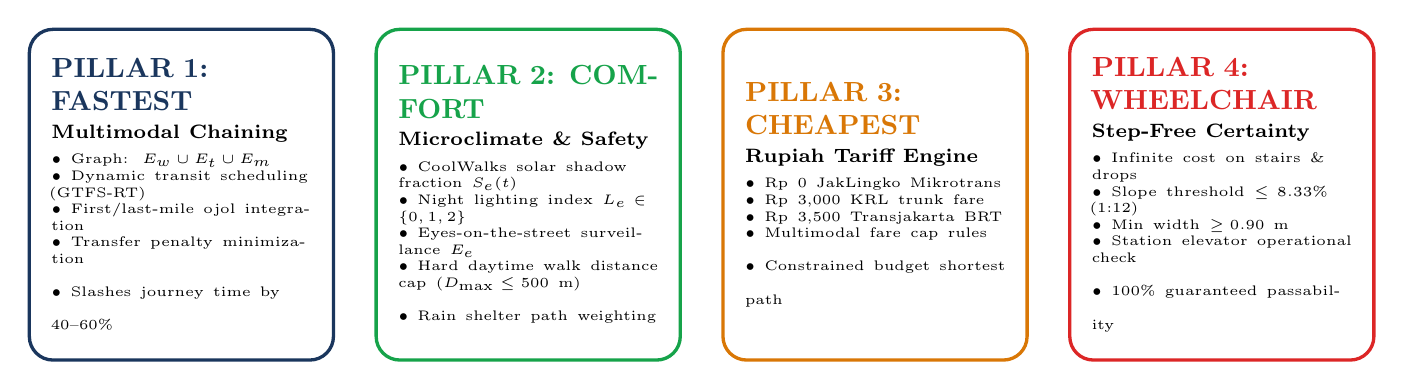
\begin{tikzpicture}[
    pillar/.style={rectangle, rounded corners=3mm, draw=pijakblue, fill=white, line width=1.2pt, text width=3.3cm, minimum height=4.2cm, align=left, inner sep=8pt},
    head/.style={font=\bfseries\color{white}, align=center},
    arr/.style={-{Stealth[length=2mm]}, line width=1pt, draw=pijakteal}
]
    % Pillar 1
    \node (p1) [pillar, draw=pijakblue] {
        \textbf{\color{pijakblue}PILLAR 1: FASTEST}\\[0.2em]
        \scriptsize\textbf{Multimodal Chaining}\\[0.4em]
        \tiny $\bullet$ Graph: $E_w \cup E_t \cup E_m$\\
        $\bullet$ Dynamic transit scheduling (GTFS-RT)\\
        $\bullet$ First/last-mile ojol integration\\
        $\bullet$ Transfer penalty minimization\\
        $\bullet$ Slashes journey time by 40--60\%
    };

    % Pillar 2
    \node (p2) [pillar, right=0.5cm of p1, draw=pijakgreen] {
        \textbf{\color{pijakgreen}PILLAR 2: COMFORT}\\[0.2em]
        \scriptsize\textbf{Microclimate \& Safety}\\[0.4em]
        \tiny $\bullet$ CoolWalks solar shadow fraction $S_e(t)$\\
        $\bullet$ Night lighting index $L_e \in \{0,1,2\}$\\
        $\bullet$ Eyes-on-the-street surveillance $E_e$\\
        $\bullet$ Hard daytime walk distance cap ($D_{\max} \le 500\text{ m}$)\\
        $\bullet$ Rain shelter path weighting
    };

    % Pillar 3
    \node (p3) [pillar, right=0.5cm of p2, draw=pijakamber] {
        \textbf{\color{pijakamber}PILLAR 3: CHEAPEST}\\[0.2em]
        \scriptsize\textbf{Rupiah Tariff Engine}\\[0.4em]
        \tiny $\bullet$ Rp~0 JakLingko Mikrotrans\\
        $\bullet$ Rp~3,000 KRL trunk fare\\
        $\bullet$ Rp~3,500 Transjakarta BRT\\
        $\bullet$ Multimodal fare cap rules\\
        $\bullet$ Constrained budget shortest path
    };

    % Pillar 4
    \node (p4) [pillar, right=0.5cm of p3, draw=pijakred] {
        \textbf{\color{pijakred}PILLAR 4: WHEELCHAIR}\\[0.2em]
        \scriptsize\textbf{Step-Free Certainty}\\[0.4em]
        \tiny $\bullet$ Infinite cost on stairs \& drops\\
        $\bullet$ Slope threshold $\le 8.33\%$ (1:12)\\
        $\bullet$ Min width $\ge 0.90\text{ m}$\\
        $\bullet$ Station elevator operational check\\
        $\bullet$ 100\% guaranteed passability
    };
\end{tikzpicture}
\caption{The 4-Pillar Algorithmic Routing Matrix addressing urban transit friction.}
\label{fig:4pillars}
\end{figure}

\subsection{Mathematical Formulation of the 4 Pillars}

\subsubsection{Pillar 1: Fastest (Multimodal Chaining Engine)}
The objective is to minimize total travel time across discrete mode transfers:
\begin{equation}
    \min_{P \subseteq E} T(P) = \sum_{e \in P \cap E_w} \frac{\text{len}(e)}{v_{\text{walk}}} + \sum_{e \in P \cap E_t} t_{\text{transit}}(e) + \sum_{e \in P \cap E_m} t_{\text{ojol}}(e) + \sum_{k \in \text{Transfers}} \tau_k
\end{equation}
where $\tau_k$ is the transfer penalty reflecting physical walking through stations, fare gate clearance, and mode headways derived from real-time feeds.

\subsubsection{Pillar 2: Comfort (Thermal Shade, Night Safety \& Walk Cap)}
Pedestrian comfort heavily depends on solar radiation during daytime and passive safety at night. The edge traversal cost is modulated by dynamic environmental attributes:
\begin{equation}
    C_{\text{comfort}}(e, t) = \text{len}(e) \times \left[ 1 + w_{\text{shade}} \cdot \big(1 - S_e(t)\big) + w_{\text{light}} \cdot (2 - L_e) + w_{\text{eyes}} \cdot (2 - E_e) + w_{\text{surf}} \cdot D_e \right]
\end{equation}
subject to the physiological distance constraint calibrated against empirical acceptable walking distances in Jakarta \cite{afkara2020walking}:
\begin{equation}
    \sum_{e \in P \cap E_w} \text{len}(e) \le D_{\max}(T_{\text{ambient}})
\end{equation}
where:
\begin{itemize}[leftmargin=1.5em]
    \item $S_e(t) \in [0, 1]$ is the time-varying shade fraction at hour $t$ (derived from CoolWalks solar ray-tracing).
    \item $L_e \in \{0, 1, 2\}$ is the illumination quality ($0 = \text{unlit}$, $1 = \text{partial/blocked by foliage}$, $2 = \text{continuous luminaire}$).
    \item $E_e \in \{0, 1, 2\}$ is passive street surveillance ($0 = \text{blank wall/empty}$, $2 = \text{active commercial frontage}$).
    \item $D_{\max}$ dynamically contracts from $800\text{ m}$ to $400\text{ m}$ when ambient temperatures exceed the $27^\circ\text{C}$ THI threshold.
\end{itemize}

\subsubsection{Pillar 3: Cheapest (Rupiah Tariff Engine)}
Unlike global transit apps that compute transit without fare logic, this pillar integrates the statutory fare structures of Greater Jakarta:
\begin{equation}
    \min_{P \subseteq E} \text{Tariff}(P) \quad \text{subject to} \quad T(P) \le \alpha \cdot T_{\text{fastest}}
\end{equation}
The tariff calculation engine enforces exact transit rules:
\begin{equation}
    \text{Tariff}(P) = \sum_{r \in \text{JakLingko}} \text{Rp } 0 + \sum_{r \in \text{KRL}} \Big(\text{Rp } 3{,}000 + \text{Rp } 1{,}000 \cdot \max\big(0, \lceil\tfrac{d_r - 25}{10}\rceil\big)\Big) + \sum_{r \in \text{TJ}} \text{Rp } 3{,}500
\end{equation}
This allows lower-income commuters to identify routes that are 100\% covered by the integrated Rp~0 JakLingko feeder network joined to Rp~3,000 KRL commuter rail.

\subsubsection{Pillar 4: Wheelchair Accessible (Strict Step-Free Topological Certainty)}
For permanent wheelchair users, comfort is not a continuous variable; a single 15-cm step represents total journey termination. The cost function acts as a strict barrier filter:
\begin{equation}
    C_{\text{wheelchair}}(e) = 
    \begin{cases}
        \infty, & \text{if } \text{has\_stairs}(e) \land \neg\text{has\_operational\_lift}(e) \\
        \infty, & \text{if } \text{slope}(e) > 8.33\% \quad (\text{exceeds 1:12 ADA / Permen PUPR 14/2017 \cite{pupr2017}}) \\
        \infty, & \text{if } \text{width}(e) < 0.90\text{ m} \quad (\text{or } < 1.85\text{ m with no passing bays}) \\
        \infty, & \text{if } \text{surface}(e) = \text{damaged} \lor \text{has\_open\_drain}(e) \\
        \text{len}(e) \cdot \big(1 + \mu \cdot \text{slope}(e)\big), & \text{otherwise}
    \end{cases}
\end{equation}

% =========================================================================
\section{Automated Computer Vision \& Remote Sensing Pipeline}
% =========================================================================

To bypass the scaling bottleneck of manual audits, we designed a scalable automated data ingestion pipeline.

\begin{figure}[H]
\centering
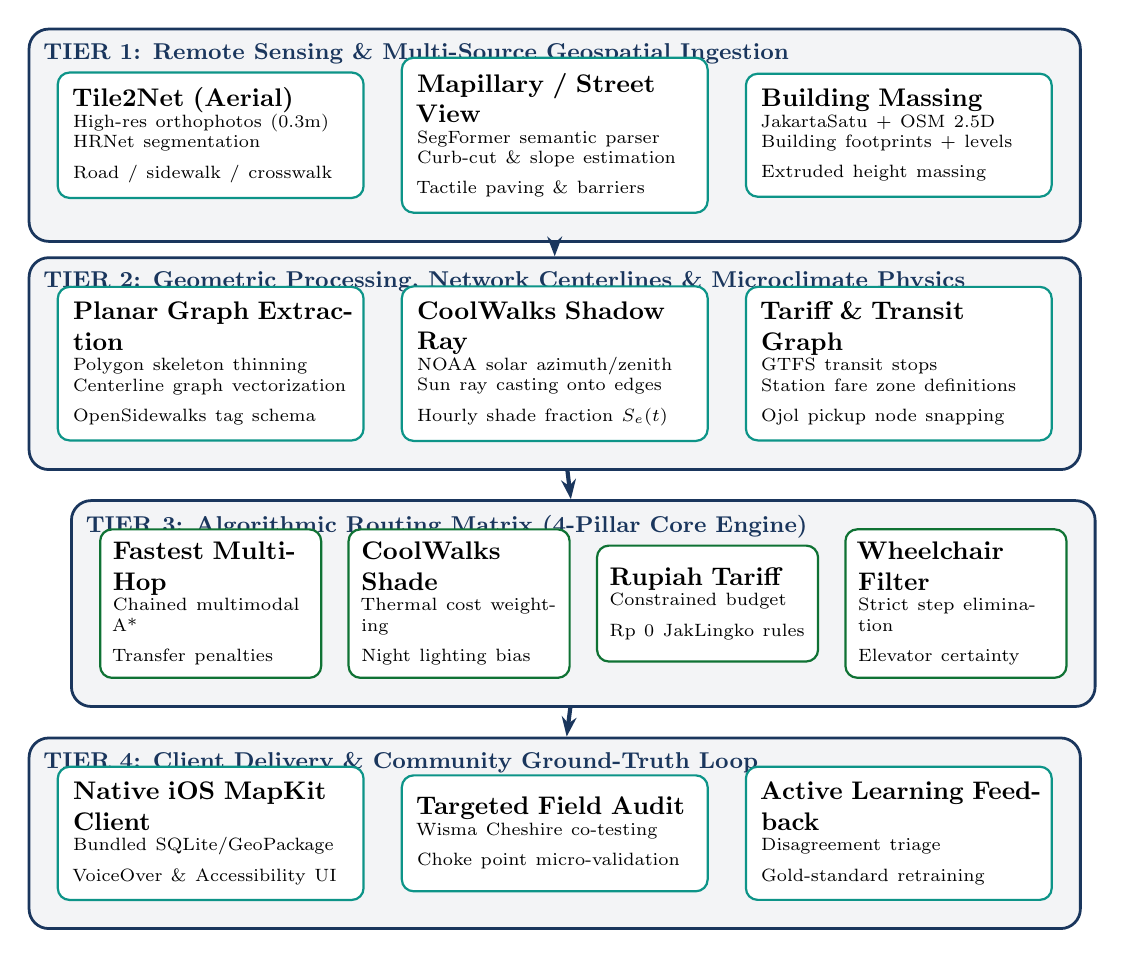
\begin{tikzpicture}[
    scale=0.92, every node/.style={transform shape},
    node distance=0.8cm and 0.5cm,
    layer/.style={rectangle, rounded corners=2.5mm, draw=pijakblue, fill=pijaklight, line width=1pt, inner sep=10pt},
    comp/.style={rectangle, rounded corners=1.5mm, draw=pijakteal, fill=white, line width=0.8pt, text width=3.8cm, minimum height=1.6cm, align=left, inner sep=6pt},
    comp3/.style={rectangle, rounded corners=1.5mm, draw=pijakgreen!70!black, fill=white, line width=0.8pt, text width=2.7cm, minimum height=1.6cm, align=left, inner sep=5pt},
    arr/.style={-{Stealth[length=2.5mm]}, line width=1.5pt, draw=pijakblue}
]
    % Tier 1
    \node (c1a) [comp] {\textbf{Tile2Net (Aerial)}\\\scriptsize High-res orthophotos (0.3m)\\HRNet segmentation\\Road / sidewalk / crosswalk};
    \node (c1b) [comp, right=0.5cm of c1a] {\textbf{Mapillary / Street View}\\\scriptsize SegFormer semantic parser\\Curb-cut \& slope estimation\\Tactile paving \& barriers};
    \node (c1c) [comp, right=0.5cm of c1b] {\textbf{Building Massing}\\\scriptsize JakartaSatu + OSM 2.5D\\Building footprints + levels\\Extruded height massing};

    \begin{scope}[on background layer]
        \node (t1) [layer, fit=(c1a) (c1b) (c1c), label={[anchor=north west, inner sep=6pt, font=\small\bfseries\color{pijakblue}]north west:TIER 1: Remote Sensing \& Multi-Source Geospatial Ingestion}] {};
    \end{scope}

    % Tier 2
    \node (c2a) [comp, below=1.2cm of c1a] {\textbf{Planar Graph Extraction}\\\scriptsize Polygon skeleton thinning\\Centerline graph vectorization\\OpenSidewalks tag schema};
    \node (c2b) [comp, right=0.5cm of c2a] {\textbf{CoolWalks Shadow Ray}\\\scriptsize NOAA solar azimuth/zenith\\Sun ray casting onto edges\\Hourly shade fraction $S_e(t)$};
    \node (c2c) [comp, right=0.5cm of c2b] {\textbf{Tariff \& Transit Graph}\\\scriptsize GTFS transit stops\\Station fare zone definitions\\Ojol pickup node snapping};

    \begin{scope}[on background layer]
        \node (t2) [layer, fit=(c2a) (c2b) (c2c), label={[anchor=north west, inner sep=6pt, font=\small\bfseries\color{pijakblue}]north west:TIER 2: Geometric Processing, Network Centerlines \& Microclimate Physics}] {};
    \end{scope}

    % Tier 3
    \node (c3a) [comp3, below=1.2cm of c2a] {\textbf{Fastest Multi-Hop}\\\scriptsize Chained multimodal A*\\Transfer penalties};
    \node (c3b) [comp3, right=0.35cm of c3a] {\textbf{CoolWalks Shade}\\\scriptsize Thermal cost weighting\\Night lighting bias};
    \node (c3c) [comp3, right=0.35cm of c3b] {\textbf{Rupiah Tariff}\\\scriptsize Constrained budget\\Rp 0 JakLingko rules};
    \node (c3d) [comp3, right=0.35cm of c3c] {\textbf{Wheelchair Filter}\\\scriptsize Strict step elimination\\Elevator certainty};

    \begin{scope}[on background layer]
        \node (t3) [layer, fit=(c3a) (c3b) (c3c) (c3d), label={[anchor=north west, inner sep=6pt, font=\small\bfseries\color{pijakblue}]north west:TIER 3: Algorithmic Routing Matrix (4-Pillar Core Engine)}] {};
    \end{scope}

    % Tier 4
    \node (c4a) [comp, below=1.2cm of c3a, text width=3.8cm] {\textbf{Native iOS MapKit Client}\\\scriptsize Bundled SQLite/GeoPackage\\VoiceOver \& Accessibility UI};
    \node (c4b) [comp, right=0.5cm of c4a, text width=3.8cm] {\textbf{Targeted Field Audit}\\\scriptsize Wisma Cheshire co-testing\\Choke point micro-validation};
    \node (c4c) [comp, right=0.5cm of c4b, text width=3.8cm] {\textbf{Active Learning Feedback}\\\scriptsize Disagreement triage\\Gold-standard retraining};

    \begin{scope}[on background layer]
        \node (t4) [layer, fit=(c4a) (c4b) (c4c), label={[anchor=north west, inner sep=6pt, font=\small\bfseries\color{pijakblue}]north west:TIER 4: Client Delivery \& Community Ground-Truth Loop}] {};
    \end{scope}

    % Connectors
    \draw [arr] (t1) -- (t2);
    \draw [arr] (t2) -- (t3);
    \draw [arr] (t3) -- (t4);
\end{tikzpicture}
\caption{End-to-End System Architecture: Automated Remote Sensing, Microclimate Modeling, and Routing.}
\label{fig:pipeline_architecture}
\end{figure}

\subsection{Tile2Net Pipeline for Southeast Asian Megacities}
\texttt{Tile2Net} (developed by NYU VIDA) utilizes deep convolutional neural networks to extract pedestrian infrastructure directly from aerial imagery \cite{tile2net2023}:
\begin{enumerate}[leftmargin=1.5em]
    \item \textbf{Tile Slicing:} Satellite and aerial orthophotos (Zoom Level 19, $\approx 0.30\text{ m/pixel}$) are retrieved from regional GIS servers (Jakarta Satu WMS and Esri World Imagery).
    \item \textbf{Semantic Segmentation:} A SegFormer/HRNet model generates probabilistic segmentation masks across four classes: \emph{roadway}, \emph{sidewalk}, \emph{crosswalk}, and \emph{footpath}.
    \item \textbf{Polygon Thinning \& Centerline Vectorization:} Morphological thinning algorithms extract medial topological axes, creating directed vector centerlines.
    \item \textbf{Regional Fine-Tuning:} Standard models trained on North American cities fail in Jakarta due to tree canopy occlusion, roadside food vendors (\emph{kaki lima}), and unpaved verges. Fine-tuning on Indonesian urban typologies is required.
\end{enumerate}

\subsection{CoolWalks Physics-Based Solar Microclimate Engine}
To compute time-varying solar shade ($S_e(t)$) without expensive 3D rendering engines, we implement the analytical solar geometry framework established by \emph{CoolWalks} \cite{coolwalks2025}:
\begin{itemize}[leftmargin=1.5em]
    \item \textbf{Solar Ephemeris Calculation:} For any latitude $\phi$, longitude $\lambda$, and timestamp $t$, solar zenith angle $\theta_z$ and solar azimuth $\alpha_s$ are computed using standard NOAA solar positioning algorithms.
    \item \textbf{2.5D Building Shadow Projection:} Building footprints are assigned heights $H = \text{levels} \times 3.2\text{ m}$. For each building polygon, a shadow extrusion polygon is projected in the direction $\alpha_s + 180^\circ$ with length:
    \begin{equation}
        L_{\text{shadow}} = \frac{H}{\tan(\theta_z)}
    \end{equation}
    \item \textbf{Segment Intersection:} The edge $e$ is spatially intersected with all cast shadow polygons. The ratio of shaded edge length to total edge length defines $S_e(t) \in [0, 1]$.
\end{itemize}

% =========================================================================
\section{How and When Do We Need Field Research?}
% =========================================================================

A central hazard in computational urban planning is \textbf{automation arrogance}---the assumption that remote sensing and machine learning can completely replace physical human inspection. Conversely, \textbf{manual audit fatigue} paralyzes projects that attempt to inspect every street meter by hand.

\begin{conceptbox}{The Golden Rule of Field Validation}
\textbf{Remote sensing provides scalable horizontal macro-coverage; field research provides deep vertical micro-truth.} Field research must never be deployed randomly. It is an expensive, high-fidelity instrument reserved exclusively for safety-critical choke points, active-learning model disputes, and participatory co-design with vulnerable user communities.
\end{conceptbox}

\begin{figure}[H]
\centering
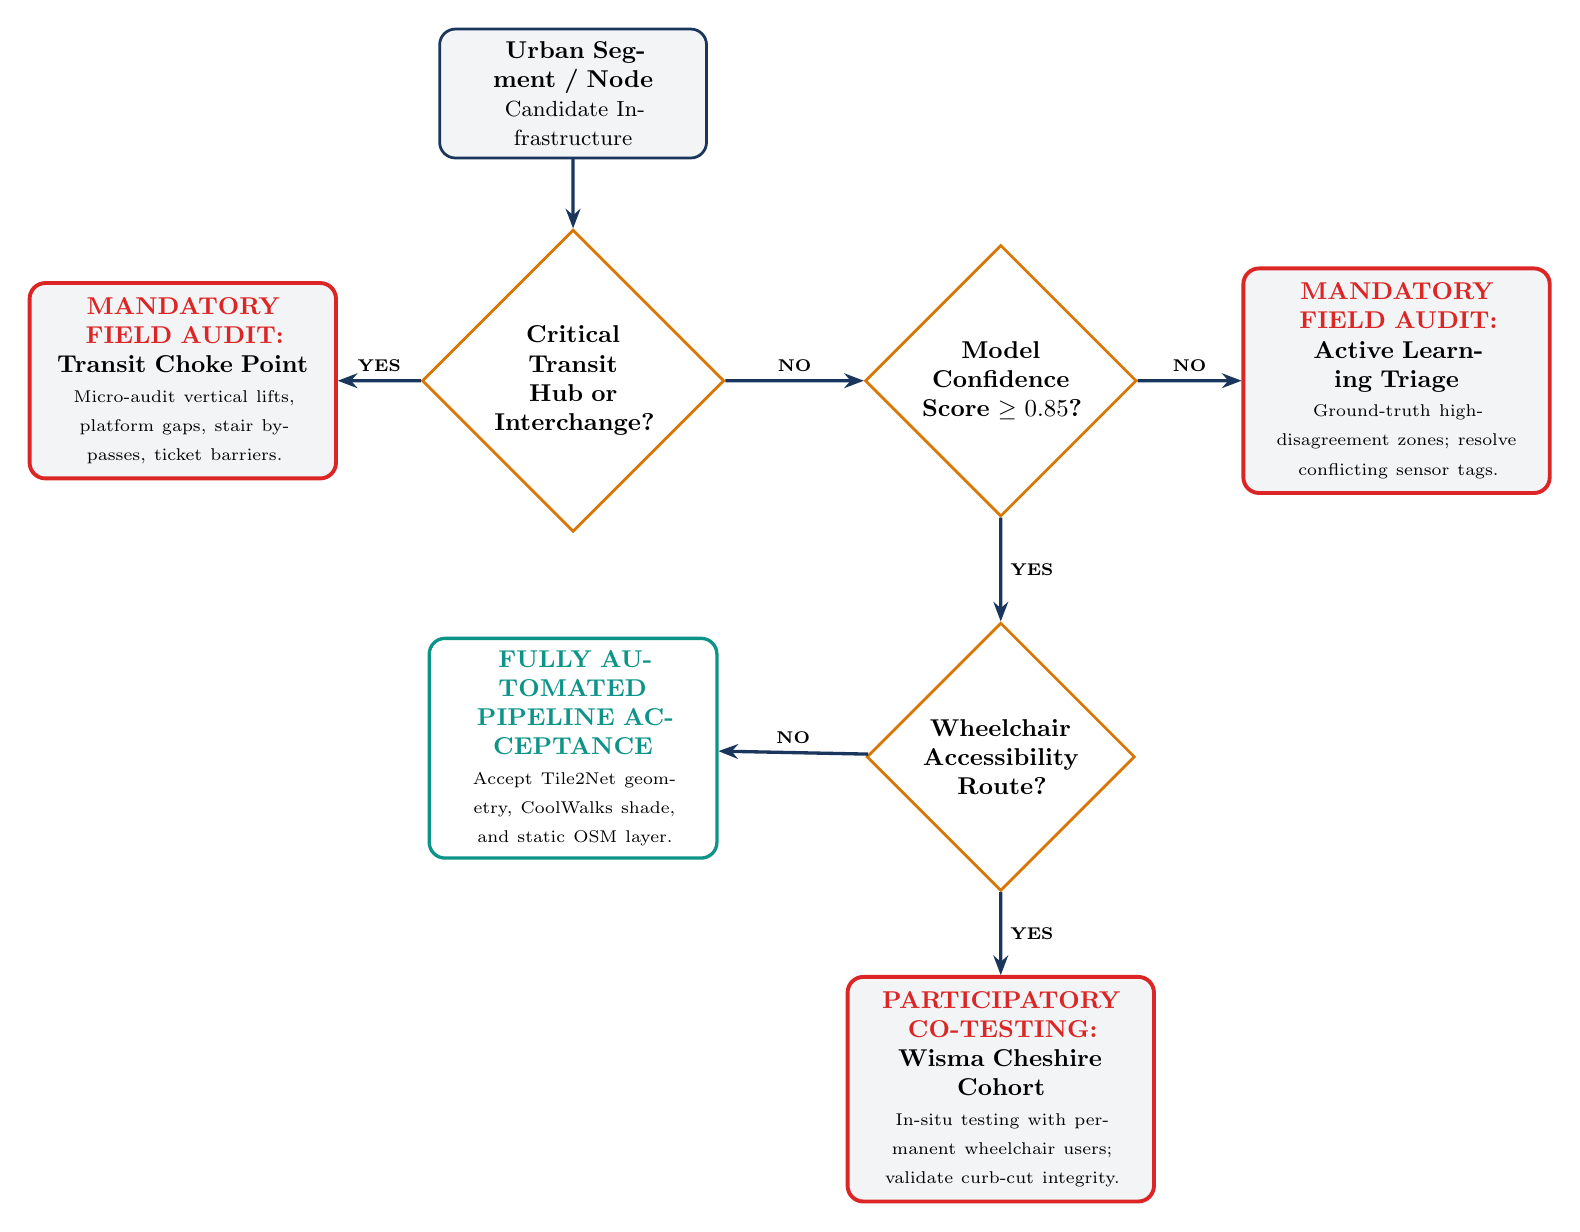
\begin{tikzpicture}[
    scale=0.88, every node/.style={transform shape},
    node distance=1.2cm and 1.5cm,
    decision/.style={diamond, draw=pijakamber, fill=white, line width=1pt, text width=2.5cm, align=center, inner sep=2pt},
    block/.style={rectangle, rounded corners=2mm, draw=pijakblue, fill=pijaklight, line width=1pt, text width=3.5cm, minimum height=1.2cm, align=center, inner sep=5pt},
    action/.style={rectangle, rounded corners=2mm, draw=pijakteal, fill=white, line width=1.2pt, text width=3.8cm, minimum height=1.3cm, align=center, inner sep=5pt},
    field/.style={rectangle, rounded corners=2mm, draw=pijakred, fill=pijaklight, line width=1.4pt, text width=4.0cm, minimum height=1.5cm, align=center, inner sep=6pt},
    arr/.style={-{Stealth[length=2.5mm]}, line width=1.2pt, draw=pijakblue}
]
    % Nodes
    \node (start) [block] {\textbf{Urban Segment / Node}\\\small Candidate Infrastructure};
    
    \node (d1) [decision, below=1.0cm of start] {\textbf{Critical Transit Hub or Interchange?}};
    
    \node (d2) [decision, right=2.0cm of d1] {\textbf{Model Confidence Score $\ge 0.85$?}};
    
    \node (d3) [decision, below=1.5cm of d2] {\textbf{Wheelchair Accessibility Route?}};

    \node (f1) [field, left=1.2cm of d1] {
        \textbf{\color{pijakred}MANDATORY FIELD AUDIT:}\\
        \textbf{Transit Choke Point}\\
        \scriptsize Micro-audit vertical lifts, platform gaps, stair bypasses, ticket barriers.
    };

    \node (f2) [field, right=1.5cm of d2] {
        \textbf{\color{pijakred}MANDATORY FIELD AUDIT:}\\
        \textbf{Active Learning Triage}\\
        \scriptsize Ground-truth high-disagreement zones; resolve conflicting sensor tags.
    };

    \node (f3) [field, below=1.2cm of d3] {
        \textbf{\color{pijakred}PARTICIPATORY CO-TESTING:}\\
        \textbf{Wisma Cheshire Cohort}\\
        \scriptsize In-situ testing with permanent wheelchair users; validate curb-cut integrity.
    };

    \node (auto) [action, below=1.5cm of d1] {
        \textbf{\color{pijakteal}FULLY AUTOMATED}\\
        \textbf{\color{pijakteal}PIPELINE ACCEPTANCE}\\
        \scriptsize Accept Tile2Net geometry, CoolWalks shade, and static OSM layer.
    };

    % Connectors
    \draw [arr] (start) -- (d1);
    \draw [arr] (d1) -- node [above, font=\scriptsize\bfseries] {YES} (f1);
    \draw [arr] (d1) -- node [above, font=\scriptsize\bfseries] {NO} (d2);
    \draw [arr] (d2) -- node [above, font=\scriptsize\bfseries] {NO} (f2);
    \draw [arr] (d2) -- node [right, font=\scriptsize\bfseries] {YES} (d3);
    \draw [arr] (d3) -- node [right, font=\scriptsize\bfseries] {YES} (f3);
    \draw [arr] (d3) -- node [above, font=\scriptsize\bfseries] {NO} (auto);
\end{tikzpicture}
\caption{Decision Flowchart: Triaging between Automated Processing and Mandatory Field Research.}
\label{fig:field_decision_flowchart}
\end{figure}

\subsection{The Operational Decision Boundary Matrix}

\begin{table}[H]
\centering
\small
\caption{Decision Boundary Matrix: Automated Remote Sensing vs. In-Situ Field Research.}
\label{tab:automation_matrix}
\renewcommand{\arraystretch}{1.2}
\begin{tabularx}{\textwidth}{p{3.5cm} p{2.2cm} p{4.5cm} p{4.5cm}}
\toprule
\textbf{Infrastructure / Phenomenon} & \textbf{Operational Mode} & \textbf{Automated Mechanism} & \textbf{Field Research Trigger \& Protocol} \\
\midrule
Regional Sidewalk Network \& Geometry & \textbf{\color{pijakteal}Automated} & Tile2Net semantic segmentation on aerial orthophotos; centerline thinning. & Only when aerial coverage is obscured by $>80\%$ persistent tree canopy or cloud cover. \\
\midrule
Solar Radiation \& Thermal Shade Layer & \textbf{\color{pijakteal}Automated} & 2.5D building extrusion + NOAA solar vector shadow ray-casting ($S_e(t)$). & Micro-calibration of local ambient temperature vs feels-like THI threshold using WeatherKit. \\
\midrule
Multi-Agency Transit Tariffs & \textbf{\color{pijakteal}Automated} & GTFS / GTFS-RT timetable parsing; statutory fare rules table (Rp 0, 3k, 3.5k). & Ticket integration rule changes; concession card validation failures. \\
\midrule
Multi-Level Transit Interchange Nodes & \textbf{\color{pijakred}Mandatory Field} & Coarse transit station point coordinates from OpenStreetMap or JakartaSatu. & \textbf{Choke Point Protocol:} Vertical elevator operating hours, ticket barrier turnstile widths, platform gaps. \\
\midrule
Wheelchair Step-Free Route Verification & \textbf{\color{pijakred}Mandatory Field} & Surface classification from Mapillary / Street View imagery. & \textbf{Wisma Cheshire Protocol:} Physical curb-ramp slope measurement, drop-off lip $>2\text{ cm}$, sewer grate gaps. \\
\midrule
Conflicting / Low-Confidence Edges & \textbf{\color{pijakred}Mandatory Field} & Active learning triage flags edges where CV model probability $<0.70$. & \textbf{Disagreement Resolution:} In-situ audit sheet deployment to create gold-standard training labels. \\
\midrule
Dynamic Social Friction (Ojol / PKL Encroachment) & \textbf{\color{pijakred}Mandatory Field} & Object detection (YOLOv8) on corridor video feeds for flow estimation. & \textbf{Behavioral Intercepts:} Peak-hour conflict audits (07:00--09:00, 17:00--19:00 WIB); night safety audits after 22:00. \\
\bottomrule
\end{tabularx}
\end{table}

\subsection{The Wisma Cheshire Co-Design \& Participatory Protocol}
The baseline prototype \emph{Pijak} was informed by caregiver interviews (Kak Ica) and accessibility experts (Ci Jessi), but lacked primary validation with permanent wheelchair users. Through our collaboration with \textbf{Wisma Cheshire Indonesia} (Jl. Wijaya Kusuma No. 15A, Cilandak Barat, South Jakarta)---a residential and vocational center for individuals with severe physical disabilities and paraplegia---we define a dedicated field research protocol:
\begin{enumerate}[leftmargin=1.5em]
    \item \textbf{Locus of Control \& Psychological Agency:} As evidenced in community research, individuals with permanent physical disabilities experience acute external locus of control induced by hostile urban architecture and chronic spatial isolation \cite{rotter1966, fakhri2025}. When a wheelchair user encounters an unexpected 20-cm curb drop or broken lift, it induces feelings of helplessness and forces them to depend on strangers carrying them---destroying personal dignity. Verified step-free routing restores internal locus of agency.
    \item \textbf{Biomechanical Fatigue Thresholds:} Manual wheelchair users expend massive upper-body energy navigating even slight gradients. Field testing measures heart-rate strain, propulsion stroke count, and tipping risks on cross-slopes exceeding 2\%, directly calibrating the slope penalty parameter $\mu$ in Pillar 4.
    \item \textbf{Curb-Cut Continuity Audits:} Testing the complete transit chain from Wisma Cheshire (Cilandak) $\rightarrow$ MRT Fatmawati $\rightarrow$ MRT Dukuh Atas $\rightarrow$ Commercial Destination. Ensuring that no single missing ramp invalidates the entire multi-kilometer journey.
\end{enumerate}

% =========================================================================
\section{Implementation Architecture \& Native Client Delivery}
% =========================================================================

\subsection{Data Separation: Engine-Agnostic Core vs. Native iOS Client}
A critical engineering architectural decision in our stack is the strict decoupling of the \textbf{Spatial Data Layer} from the \textbf{Render and Routing Client}:
\begin{itemize}[leftmargin=1.5em]
    \item \textbf{Data Pipeline (Spatial Repo):} Operates in Python (GeoPandas, Shapely, NetworkX, Tile2Net). Emits highly optimized, planarized GeoJSON and bundled SQLite / GeoPackage files containing precomputed shade fractions ($S_e(t)$) and accessibility metadata.
    \item \textbf{Native Client (Pijak iOS):} Implemented in native Swift 6 and SwiftUI utilizing Apple MapKit (\texttt{MKOverlay}, \texttt{MKPolyline}). Avoids heavy cross-platform 3D runtimes (Unity) which consume 50+ MB of binary overhead and severely degrade device battery life.
    \item \textbf{Accessibility Compliance:} Leveraging native MapKit guarantees full system integration with Apple VoiceOver, Dynamic Type, and Apple Watch Wheelchair Workout metrics out of the box.
\end{itemize}

\subsection{Anti-Spam Defense for Indonesian Geospatial Data}
During the July 2026 deployment of \emph{Pijak}, field testing across Jakarta uncovered widespread geospatial database pollution (fraudulent commercial pins, duplicate online gambling anchors, and commercial spam placed at city centroid coordinates). To ensure data integrity, our pipeline enforces a three-tier defensive filter:
\begin{enumerate}[leftmargin=1.5em]
    \item \textbf{Centroid Co-location Filter:} If more than 3 distinct commercial POIs share identical latitude and longitude down to 5 decimal places, the cluster is flagged as synthetic spam and purged.
    \item \textbf{String Heuristic Sanitizer:} Automated regex filtering removes promotional strings containing telephone numbers, promotional gambling keywords, or unnatural punctuation strings.
    \item \textbf{Spatial Drift Bounding:} When reconciling Apple Maps POIs with Google Places accessibility metadata, associations are strictly rejected if the Euclidean distance between candidate pins exceeds 500 meters.
\end{enumerate}

% =========================================================================
\section{Strategic Roadmap, Policy Impact \& Collaborative Next Steps}
% =========================================================================

\subsection{15-Day Immediate Execution Roadmap (Investigate / Engage)}
\begin{itemize}[leftmargin=1.5em]
    \item \textbf{Days 1--4 (Overleaf Review \& Literature Sync):} Distribute this concept paper to academic mentors and municipal research partners (Karsa City Lab, ITDP Indonesia, FTDJ). Consolidate comments.
    \item \textbf{Days 5--8 (Targeted Wisma Cheshire In-Situ Session):} Conduct structured mobility walkthroughs with 3--5 manual wheelchair residents along the MRT Fatmawati--Dukuh Atas corridor. Log exact biomechanical and elevation friction points.
    \item \textbf{Days 9--12 (Tile2Net Jakarta Fine-Tuning):} Annotate 200 high-resolution aerial tiles of South Jakarta (Cilandak, Blok M, Sudirman) to fine-tune the SegFormer semantic segmentation model.
    \item \textbf{Days 13--15 (Algorithmic Routing Prototype):} Integrate the 4-pillar cost functions into an interactive web dashboard and mobile TestFlight build for user feedback.
\end{itemize}

\subsection{Institutional \& Policy Engagement}
Our research architecture directly provides actionable spatial intelligence for municipal governance:
\begin{enumerate}[leftmargin=1.5em]
    \item \textbf{Dinas Perhubungan (Dishub) DKI Jakarta:} Providing the first quantitative Walkability Gradient dataset (Table~\ref{tab:gradient_comparison}) to prioritize municipal sidewalk capital budgets in back-street kampung connectors rather than repeatedly re-paving existing arterial boulevards.
    \item \textbf{MRT Jakarta \& PT Moda Integrasi Transportasi Jabodetabek (MITJ):} Supplying verified step-free transfer graphs to eliminate multi-operator jurisdictional voids at major transit interchanges.
    \item \textbf{Civil Society \& DPOs (Wisma Cheshire, JBFT):} Empowering disability advocacy organizations with open, citable spatial data to hold municipal agencies accountable under Law No. 8/2016 on Persons with Disabilities.
\end{enumerate}

% =========================================================================
%   STANDALONE BIBLIOGRAPHY (Overleaf Self-Contained)
% =========================================================================
\begin{thebibliography}{99}

\bibitem{itdp2019}
Institute for Transportation and Development Policy (ITDP),
\emph{Panduan Desain Fasilitas Pejalan Kaki di Kawasan Transit Jakarta},
ITDP Indonesia Technical Report, Jakarta, 2019.

\bibitem{goodstats2024}
GoodStats,
``Potret Mobilitas Komuter Jabodetabek: Ketergantungan Kendaraan Pribadi dan Tantangan Angkutan Massal,''
\emph{Data Komuter BPS \& GoodStats Urban Brief}, Jakarta, 2024.

\bibitem{afkara2020walking}
M.~R. Afkara and D.~Kusuma,
``Willingness to Walk and Acceptable Walking Distances to Transit-Oriented Development Nodes in Jakarta,''
\emph{Journal of Sustainable Urban Mobility}, vol.~8, no.~2, pp.~112--126, 2020.

\bibitem{dwisadana2024}
A.~Dwisadana and B.~S. Kombaitan,
``Evaluation of Pedestrian Environment Quality Index (PEQI) on Revitalized Sidewalks: Case of South Sudirman Corridor,''
\emph{Indonesian Journal of Spatial Planning}, vol.~12, no.~1, pp.~45--58, 2024.

\bibitem{mulyadi2022}
A.~Mulyadi,
``Impact of Road-Diet Policy and Sidewalk Expansion on Public Transport Ridership in Jakarta,''
\emph{Urban Transport Review}, vol.~19, no.~3, pp.~201--215, 2022.

\bibitem{ridhani2015}
F.~Ridhani,
\emph{Global Walkability Index Assessment of Central Jakarta Commercial Corridors},
Master's thesis, Institut Teknologi Bandung, 2015.

\bibitem{apritasari2020satisfaction}
D.~Apritasari,
``Pedestrian Satisfaction on Street Furniture and Signage of Sudirman-Thamrin Corridor,''
\emph{Journal of Urban Design and Heritage}, vol.~4, no.~2, pp.~89--104, 2020.

\bibitem{rakhmatulloh2020}
A.~R. Rakhmatulloh and D.~I. Kusumo,
``Travel Characteristics and Pedestrian Access at the Dukuh Atas Transit Nexus,''
\emph{IOP Conf. Series: Earth and Environmental Science}, vol.~447, p.~012015, 2020.

\bibitem{napitupulu2025tod}
S.~Napitupulu and I.~Rudiarto,
``Post-MRT Walkability Assessment: A 400-Meter Catchment Analysis at Dukuh Atas TOD,''
\emph{Cities \& Infrastructure}, vol.~31, pp.~104--119, 2025.

\bibitem{coolwalks2025}
H.~Wolf, A.~R. Vier\o, and M.~Szell,
``CoolWalks for active mobility in urban street networks,''
\emph{Scientific Reports}, vol.~15, no.~1, p.~14911, 2025.

\bibitem{tile2net2023}
M.~Hosny, N.~Gao, and C.~Silva,
``Tile2Net: A deep learning framework for semantic extraction of pedestrian infrastructure from aerial tiles,''
\emph{Computers, Environment and Urban Systems}, vol.~104, p.~102001, 2023.

\bibitem{rotter1966}
J.~B. Rotter,
``Generalized expectancies for internal versus external control of reinforcement,''
\emph{Psychological Monographs: General and Applied}, vol.~80, no.~1, pp.~1--28, 1966.

\bibitem{fakhri2025}
M.~Fakhri, S.~Pratama, and R.~Nurul,
``Digital Hyperconnectivity and Urban Loneliness: Empirical Evidence from Indonesian Young Adults,''
\emph{Asian Journal of Social Psychology}, vol.~28, no.~2, pp.~145--162, 2025.

\bibitem{pupr2017}
Kementerian Pekerjaan Umum dan Perumahan Rakyat (PUPR),
\emph{Peraturan Menteri PUPR No. 14/PRT/M/2017 tentang Persyaratan Kemudahan Bangunan Gedung (Aksesibilitas dan Fasilitas Disabilitas)},
Jakarta, 2017.

\end{thebibliography}

\end{document}
